\section{Extrinsic calibration}

\begin{figure}[h]
  \centering
  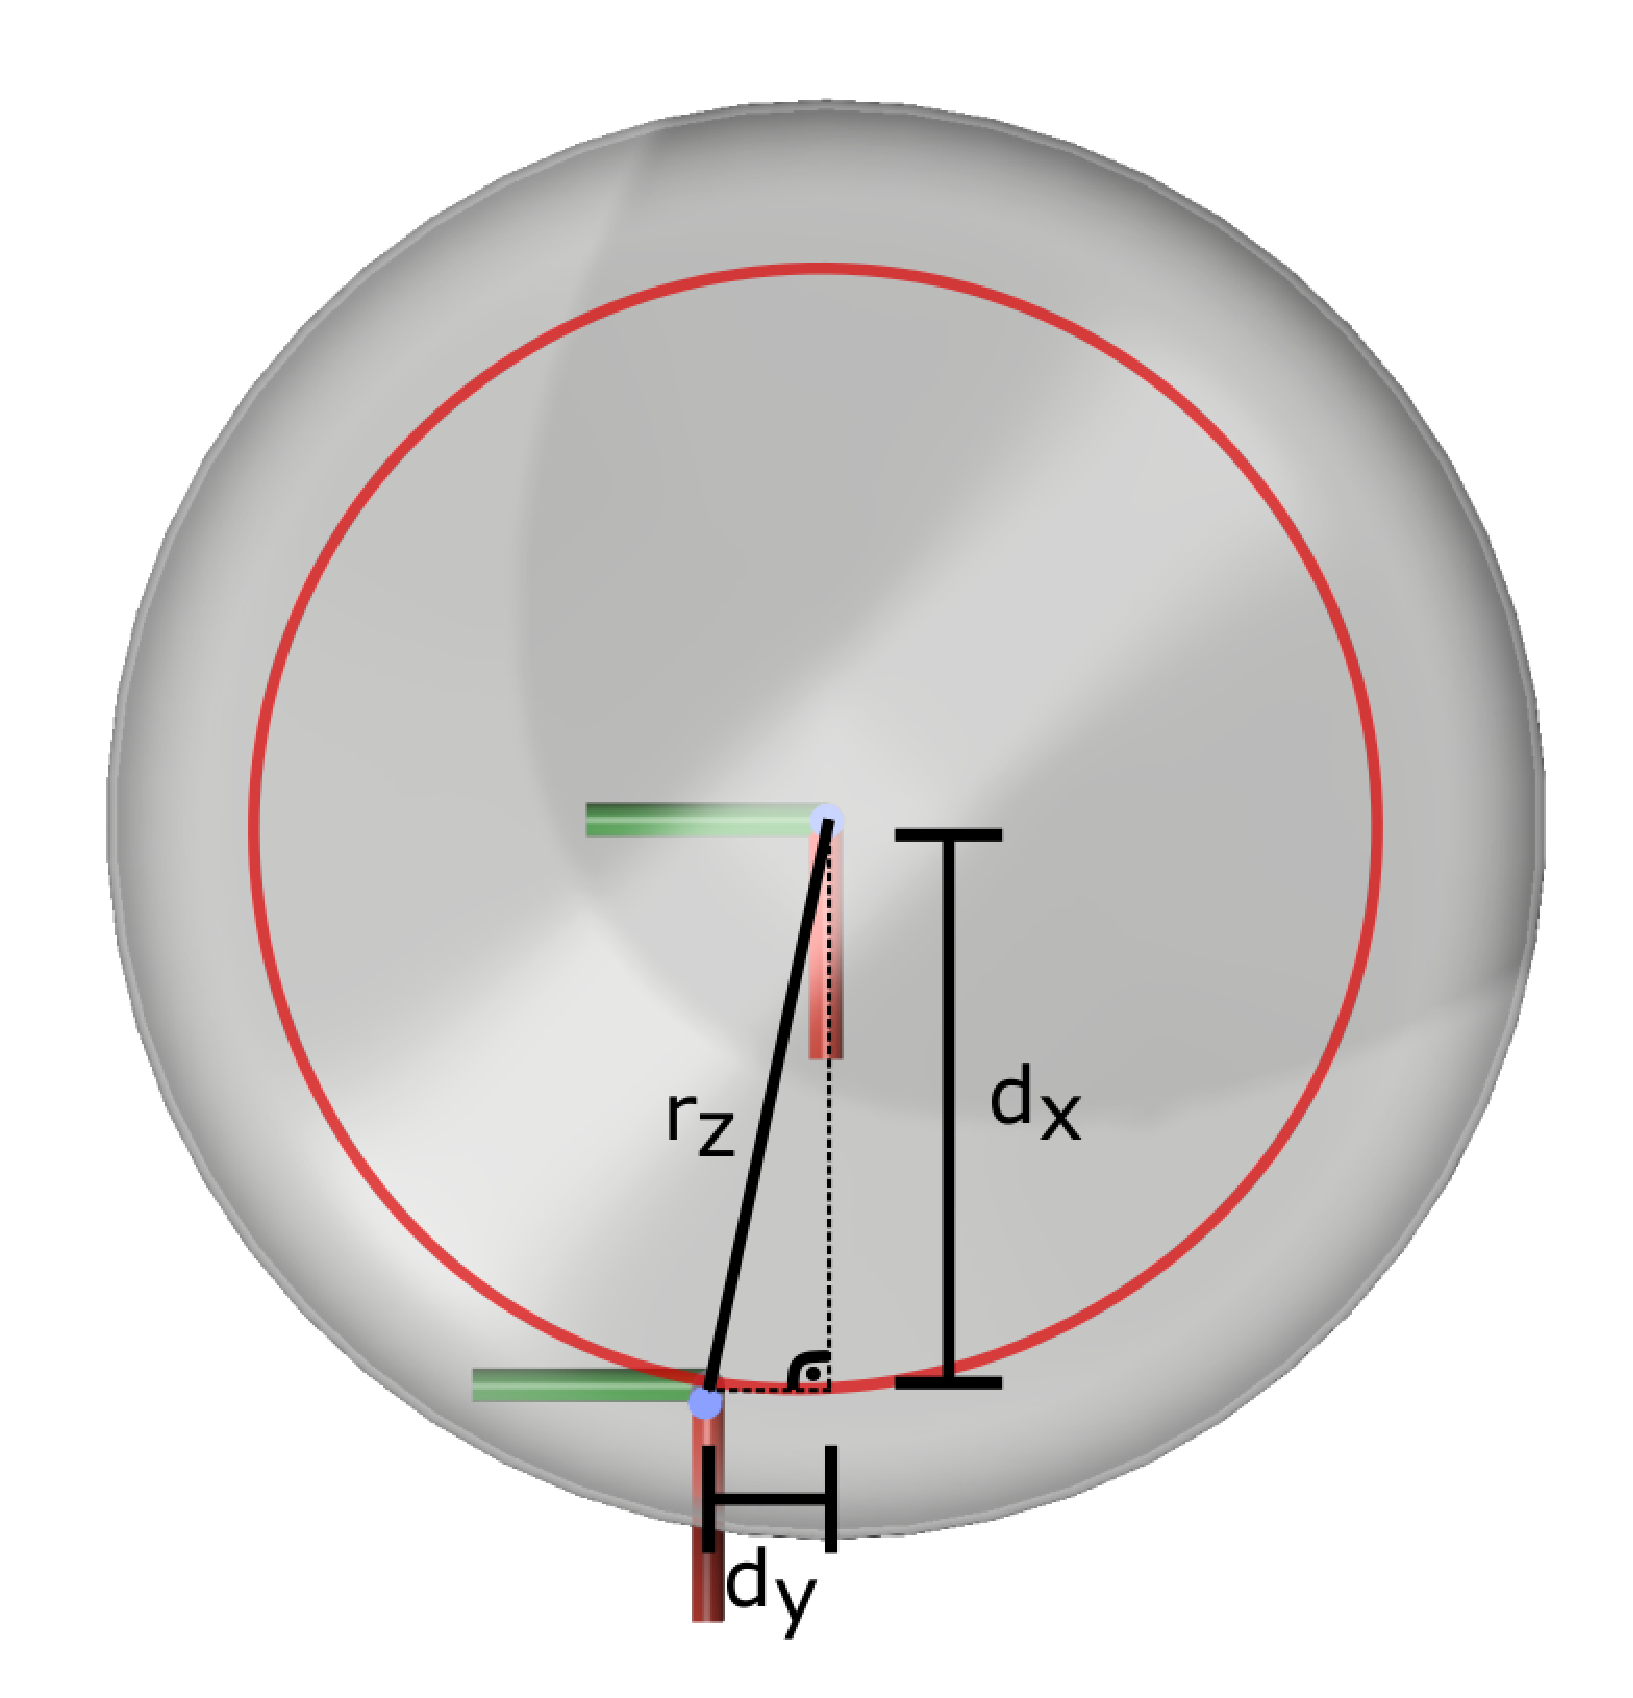
\includegraphics[width=.5\linewidth]{img/calibsphere}
  \caption{Calibration principle of a sensor inside a ball, illustrated in one axis.}
  \label{fig:calibsphere}
\end{figure}

The sensor, when mounted off-centered in the ball, will make circular trajectories if the ball rotates around an axis through its center.
We measure the radii of the sensor around the three orthogonal principal axes, which is enough information to construct the extrinsic parameters, describing the offset to the balls center.